\documentclass[amscd, amssymb, verbatim]{amsart}[12pt]

\usepackage{amsmath,amssymb,amsthm}
\usepackage[utf8]{inputenc}
\usepackage{graphicx}
\usepackage{fullpage}
\usepackage[colorlinks,linkcolor=blue,urlcolor=blue,citecolor=blue,destlabel=true]{hyperref}
\usepackage{placeins}
\usepackage[ruled,vlined]{algorithm2e}

\newcommand{\note}[1]{\textcolor{blue}{({#1})}}

\theoremstyle{plain}
\newtheorem{lemma}{Lemma}[section]
\newtheorem{theorem}[lemma]{Theorem}
\newtheorem{fact}[lemma]{Fact}
\newtheorem{corollary}[lemma]{Corollary}
\newtheorem{proposition}[lemma]{Proposition}
\newtheorem{conjecture}[lemma]{Conjecture}
\newtheorem{problem}[lemma]{Problem}
\newtheorem{claim}[lemma]{Claim}
\theoremstyle{definition}
\newtheorem{definition}[lemma]{Definition}
\newtheorem{example}[lemma]{Example}
\newtheorem{question}[lemma]{Question}
\newtheorem{remark}[lemma]{Remark}

\newcommand{\N}{\mathbb{N}}
\newcommand{\R}{\mathbb{R}}
\newcommand{\Z}{\mathbb{Z}}
\newcommand{\cB}{\mathcal{B}}
\newcommand{\cone}{\mathrm{Cone}}
\newcommand{\conv}{\mathrm{conv}}
\DeclareMathOperator{\cl}{Cl}

\begin{document}

\title{
A survey of the planar wedge of spheres conjecture
%On the minimal cores of unit disk graphs
% Planar Vietoris--Rips complexes are wedges of spheres
}
\author{CSU Putnam Seminar, Spring 2019 (we will add our names later)}
\date{\today}
\maketitle

\note{You can type any comments or ask questions in a blue ``note" environment!}

\section{Introduction}

A recent conjecture states that the clique complex of any unit disk graph is a wedge of spheres (up to homotopy type).
\begin{conjecture}\label{conj:main}
The clique complex of any unit disk graph is homotopy equivalent to a wedge sum of spheres.
\end{conjecture}
An equivalent formulation is that the Vietoris--Rips complex of any set of points in the plane is a wedge of spheres.
We will survey what is known and not known about this conjecture, and also describe some related computational experiments.

\cite{AFV,chambers2010vietoris}


\section{Project Overview}

The wikipedia article \url{https://en.wikipedia.org/wiki/Cop-win\_graph} explains a game of pursuit evasion on a graph $G$, where a robber is trying to evade a cop. 
We say that a graph $G$ is \emph{cop-win} if, no matter where the cop and robber are placed initially, the cop can always catch the robber.

It turns out that a graph $G$ is a cop-win graph if and only if it is \emph{dismantlable}, which we will describe in Section~\ref{sec:cop-win}.
Roughly speaking, a graph is dismantlable if you can ``remove dominated vertices" until you end up with only a single vertex.
More generally, after you have removed as many dominated vertices as possible, the resulting graph is called a \emph{minimal core}. Surprisingly, it turns out that all possible minimal cores of a graph are isomorphic to each other.

In this project, we will study the minimal cores of unit disk graphs.
A unit disk graph is a very particular type of graph which is formed by selecting a finite set of vertices in the plane $\R^2$, and then connecting two vertices by an edge if and only if the Euclidean distance between them is at most one.

The minimal cores of unit disk graphs from points on the circle are already classified.
Roughly speaking, one of our main questions will be to explore whether unit disk graphs from points in $\R^2$ are ``simple combinations" of unit disk graphs from points on the circle, or if the unit disk graphs from arbitrary points in $\R^2$ can exhibit ``wildly new phenomena."

One of our first tasks will be to learn the basics of cop-win graphs.

A major task will be to write software that can accept an arbitrary graph as input, and then as output return a minimal core.
We can test this software on unit disk graphs from the circle.
We will then use this software to visualize unit disk graphs of points in $\R^2$.

A later task will be to learn a little bit of combinatorial topology.
Part of the motivation for this project is to prove or disprove the conjecture that ``the clique complex of the unit disk graph of any finite set of points in $\R^2$ is always homotopy equivalent to a wedge sum of spheres", whatever in the world that means!

\cite{Bjorner1995,Carlsson2009,EdelsbrunnerHarer,edelsbrunner2000topological,Hatcher,Hausmann1995}

\section{Cop-win graphs}\label{sec:cop-win}

Let $G=(V,E)$ be a simple undirected graph (no loops or multiple edges) with $V$ the set of vertices and with $E$ the set of edges.

For any vertex $v\in V$, let $N[v]=\{v\}\cup\{u\in V~|~uv\in E\}$ be the \emph{closed neighborhood} of $v$ (where ``closed" implies that the vertex $v$ is itself included in this neighborhood).
\begin{definition}\label{def:dominated}
In a graph $G$, we say that a vertex $v$ is \emph{dominated} by a vertex $u$ if $N[v]\subseteq N[u]$.
\end{definition}

\begin{figure}[h]
\centering
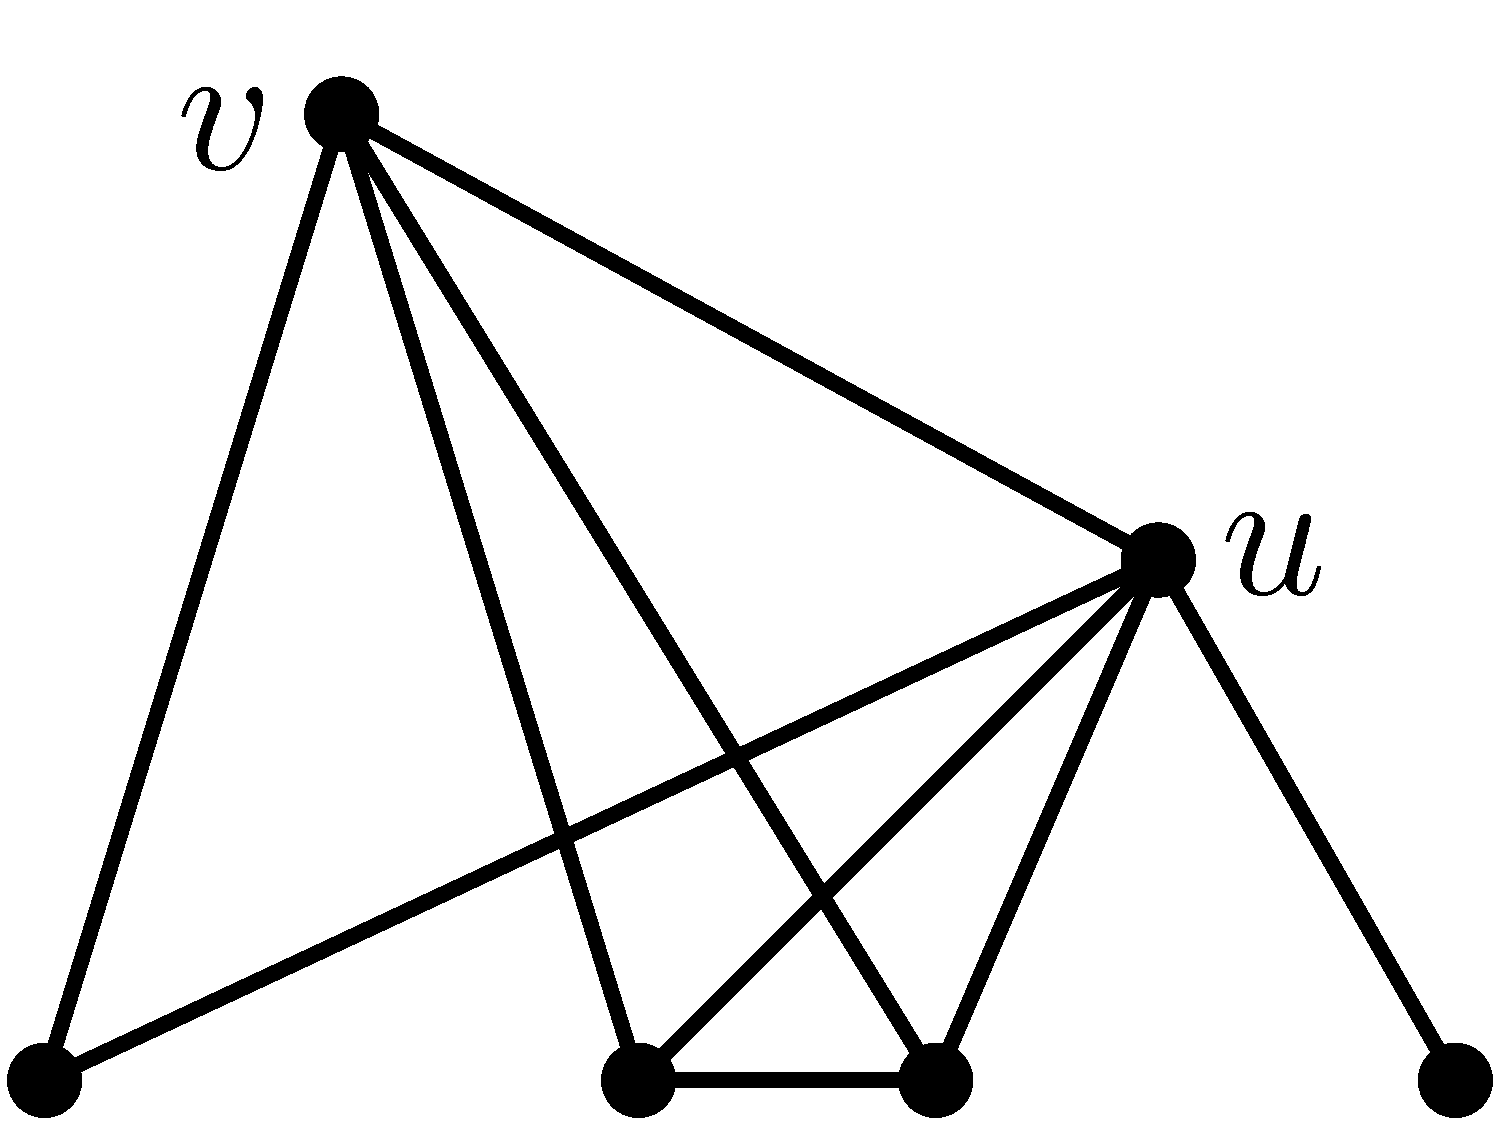
\includegraphics[width=0.2\textwidth]{Dominated1_labeled.pdf}
\caption{Vertex $v$ is dominated by vertex $u$.}
\label{fig:dominated}
\end{figure}

%Let $G\setminus u$ be the graph obtained by deleting $u$ and all of the edges containing $u$.

If you iteratively remove dominated vertices from a graph $G$, then your final ending configuration (once there are no more remaining dominated vertices) is called a \emph{minimal core}.
An important fact is that all minimal cores of a graph are isomorphic.

We say that a graph $G$ is \emph{dismantlable} if its minimal core is a single vertex, or equivalently, if one can remove dominated vertices one-by-one until only a single vertex remains.
A second important fact is that a graph is a cop-win graph if and only if it is dismantlable.



\section{Algorithms for computing minimal cores}
See \url{https://en.wikipedia.org/wiki/Cop-win\_graph} for some information on algorithms computing the minimal core of a graph.
What software options are out there, and should we write our own?
The main place to look is google!
Two other places to look are sage and polymake.

I claim that if we wish to implement it ourselves, the ``right'' way to do it is to implement the graph data structure in (\footnote{\url{https://www.sciencedirect.com/science/article/pii/S0304397511009662?via\%3Dihub}}), because it will help time bounds greatly for finding dominated vertices.  It does look kinda complicated, but that paper has everything we would need. 

% Useless trivia: If you remove a dominated vertex from a graph, no dominated vertices will become un-dominated.  However, new dominated vertices \emph{may} be created.  Thus, a simple greedy algorithm (e.g. while there exists a dominated vertex, remove it) will not return incorrect results.


\section{Unit disk graphs}

Let $\R^2$ be the euclidean plane, and for any two points $u,v\in\R^2$, let $d(u,v)$ denote the Euclidean distance between them.

\begin{definition}
Let $V \subseteq \R^2$ be a subset of the plane.
The \emph{unit disk graph} $G(V)$ is the graph $G$ with vertex set $V$, in $u,v$ are the vertices of an edge in $G(V)$ if and only if $d(u,v) \leq 1$.
\end{definition}

Given $V\subseteq \R^2$ of size $n$, how does one compute the unit disk graph $G(V)$?
The na\"{i}ve algorithm is to iterate over all $\binom{n}{2}$ pairs of vertices, to compute the distance between them, and then to include $uv$ as an edge if and only if $d(u,v)\le1$.
In Algorithm~\ref{alg:udg} we give a fancier algorithm, in which we first sort the vertices of $V$ into unit square boxes, and then only search for edges between vertices in the same or adjacent boxes.
Algorithm~\ref{alg:udg} has the same worst-case $O(n^2)$ running time as the na\"{i}ve algorithm, but will be more efficient when the vertex set is not very dense (relative to the unit scale).

\begin{algorithm}[ht]
\SetAlgoLined
\KwData{Vertex set $V(\vec{x},\vec{y})\subseteq\R^2$}
\KwResult{Edges of the unit disk graph $G(V)$}
($x_\text{min}, y_\text{min}$) = ($\min\vec{x},\min\vec{y}$)\;
%($x_\text{max}, y_\text{max}$) = ($\max\vec{x},\max\vec{y}$)\;
divide $\R^2$ into square boxes of side-length 1\;
\For{$v \in V$}{
$[i,j]$ = $\left\lfloor x - x_\text{min}, y - y_\text{min}\right\rfloor$\;
}
\For{all boxes}{
compute $d(u,v)$ among all points in this box and all immediate neighbors\;
}
\caption{Computing a unit disk graph}
\label{alg:udg}
\end{algorithm}

\note{Does somebody want to write software that will accept as input a set of points in the plane, and then compute its unit disk graph?
The na\"{i}ve algorithm would be easier than Algorithm~\ref{alg:udg} as an initial first step, though either algorithm would be great!}



\section{Minimal cores of unit disk graphs on the circle}

\note{These are classifiable---we will describe.}

\note{Does somebody want to take a stab at describing these ``$C_n^k$" graphs?}

\begin{definition}
The graph $C_n^k$ has $n$ vertices, $v_1, v_2, \ldots, v_n$. There is an edge $v_iv_j$ iff $|i - j| \leq k$.
\end{definition}

\cite{Adamaszek2013,AA-VRS1,AAFPP-J}


\section{Minimal cores of unit disk graphs in the plane}

\note{This is where we will be doing much of our initial exploring/work!}



\section{Questions}

Are the minimal cores of unit disk graphs in the plane ``simple combinations" of unit disk graphs from points on the circle, or can they exhibit ``wildly new phenomena"?

\note{After experiments, we may find some new phenomena that we try to collapse down via other techniques --- see Section~\ref{sec:collapse}.}



\section{Voronoi diagrams and Delaunay triangulations}

\note{Does somebody want to start briefly describing Voronoi diagrams and Delaunay triangulations?
Steal (and cite) an image from wikipedia, as done also in Figure~\ref{fig:simplicialComplex}. The point is that these may guide which parts of the complex we try to collapse.}



\section{Related references: non-topological}

Related references for the non-topological aspects of this project include the following.
The original paper appears to be~\cite{aigner1984game}, available at (\footnote{\url{https://www.math.ucdavis.edu/~erikslivken/classes/2016\_spring\_180/aigner\%20fromme.pdf}}). There is also a book~\cite{bonato2011game} by the author of (\footnote{\url{http://www.math.ryerson.ca/~abonato/papers/conjectures\_CR\_jan18\_2015.pdf}}). See the webpages (\footnote{\url{https://users.auth.gr/kehagiat/Research/CopRob/index.htm}}), (\footnote{\url{http://math.ucsd.edu/~fan/152/arch/coprob/}}), (\footnote{\url{https://www.mathworks.com/matlabcentral/fileexchange/31774-cops-and-robber-software}}), and the references within. See also (\footnote{\url{https://arxiv.org/pdf/1108.2549.pdf}}), (\footnote{\url{https://www.cambridge.org/core/journals/combinatorics-probability-and-computing/article/cops-and-robbers-on-geometric-graphs/22DA76A41397162164E755B52D6C3D81}}), (\footnote{\url{https://www.universiteitleiden.nl/binaries/content/assets/science/mi/scripties/master/2017-2018/mark-van-den-bergh-08-09-2017.pdf}}).



\section{Related references: topological}

\cite{chambers2010vietoris}

Paper by Adamasek, Frick, Vakili



\section{The topological perspective}

Recall that a graph is a collection of vertices (0-dimensional pieces) and edges (1-dimensional pieces) that are ``glued-together compatibly".
What if we now also allow triangles (2-dimensional pieces), tetrahedra (3-dimensional pieces), etc? The resulting object is called a \emph{simplicial complex}; see for example \url{https://en.wikipedia.org/wiki/Simplicial\_complex}. 
Instead of calling these pieces vertices, edges, triangles, tetrahedra, etc, we can more efficiently call them $k$-simplices, where $k$ is the dimension of the piece!
For example, a vertex is a 0-simplex, an edge is a 1-simplex, a triangle is a 2-simplex, and a tetrahedron is a 3-simplex. Note that a $k$-simplex is a $k$-dimensional building block consisting of $k+1$ vertices. The advantage of this notation is that now we can also talk about $k$-simplices for any $k\ge 0$!
Though some definitions of simplicial complexes feel a little abstract, the right perspective is to think of a simplicial complex as a LEGO set that is formed by gluing simple building blocks (simplices) together!

\begin{definition}
A \emph{simplicial complex} $K$ on a vertex set $V$ is a set of simplices $\sigma \subseteq V$, such that if $\sigma\in K$ (meaning $\sigma$ is a simplex in the complex) and $\tau\subseteq\sigma$ (meaning $\tau$ is a face of $\sigma$), then we also have $\tau\in K$ (meaning that $\tau$ is also a simplex in the complex).
\footnote{Strictly speaking, if we we want to say that $V$ is the vertex set of $K$, then we should also specify that each singleton element of $V$ is a simplex in $K$.}
\end{definition}

\begin{figure}[h]
\centering
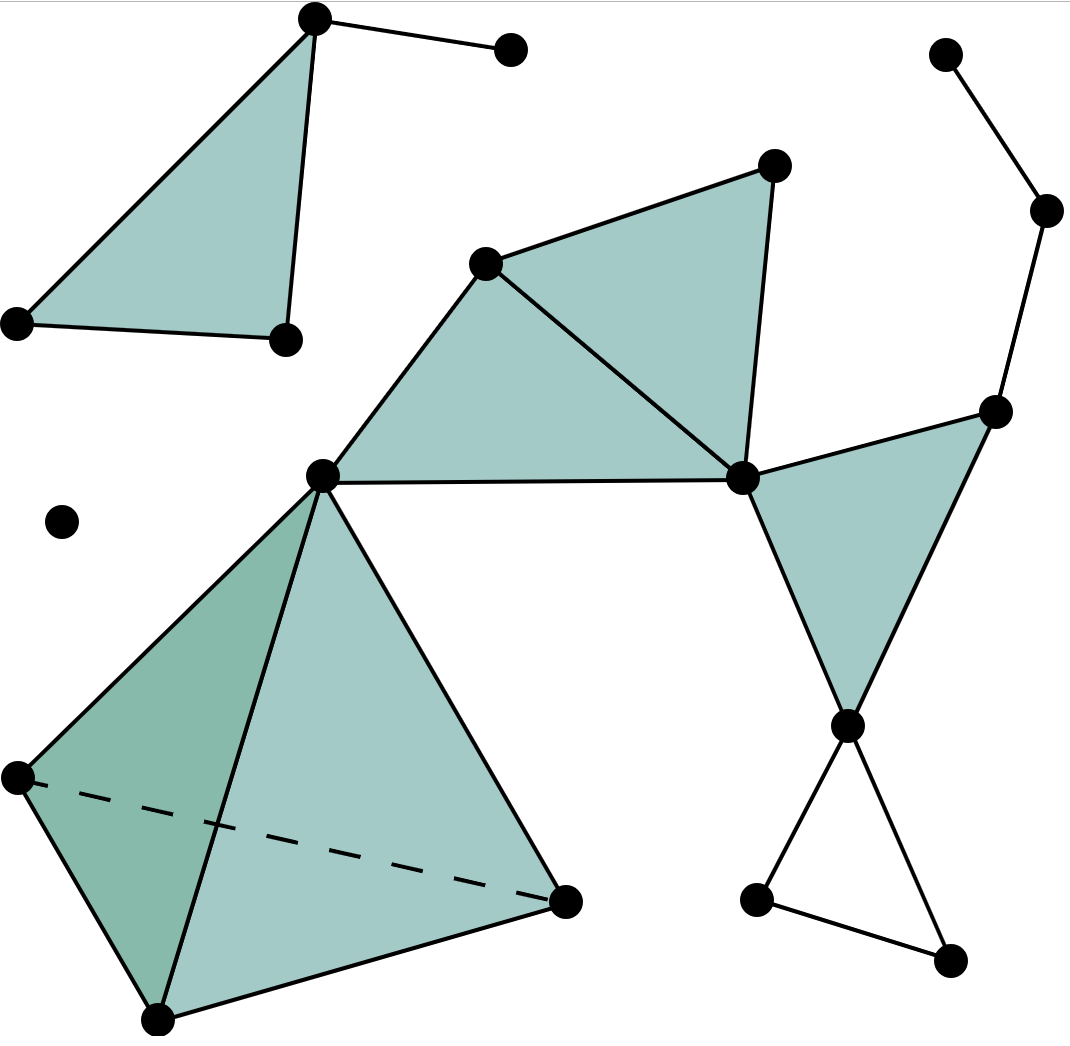
\includegraphics[width=0.2\textwidth]{SimplicialComplex.png}
\hspace{20mm}
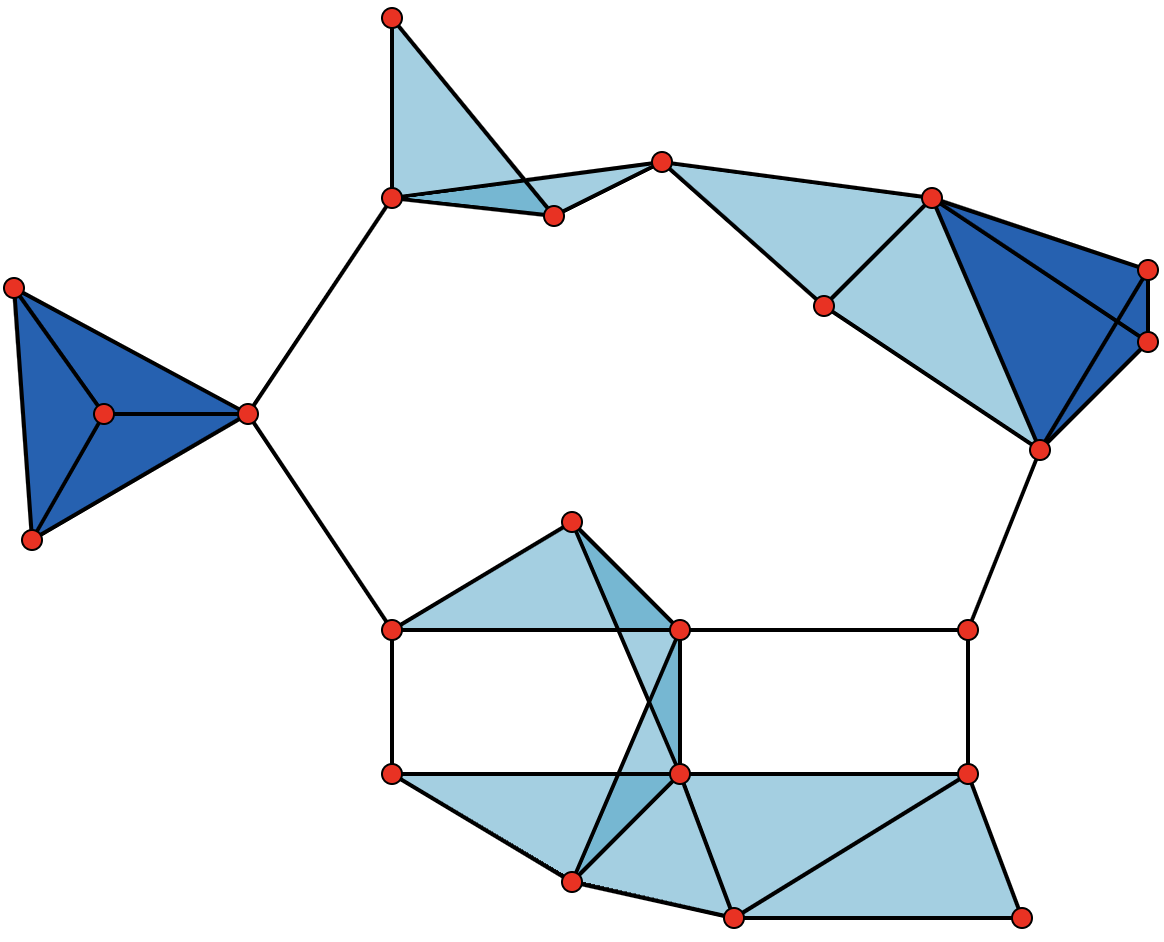
\includegraphics[width=0.25\textwidth]{CliqueComplex.png}
\caption{(Left) A simplicial complex. (Right) A clique complex.
Note the leftmost figure is not a clique complex since it has an empty triangle!
Both figures are from Wikipedia.}
\label{fig:simplicialComplex}
\end{figure}

A \emph{clique complex} is a way to build a simplicial complex on top of a graph; see for example \url{https://en.wikipedia.org/wiki/Clique\_complex}.
More specifically, let $G=(V,E)$ be a simple undirected graph (no loops or multiple edges) with $V$ the set of vertices and with $E$ the set of edges.

\begin{definition}
The \emph{clique complex $\cl(G)$} of a graph $G=(V,E)$ is the largest simplicial complex that has $V$ as its set of vertices and $E$ as its set of edges.
That is, $\cl(G)$ contains $\{v_0,\ldots,v_k\}\subseteq V$ as a simplex if $v_iv_j\in E$ (i.e.\ if $v_iv_j$ is an edge in $G$) for all $0\le i,j\le k$.
\end{definition}

\begin{definition}
Given a metric space $X$ and a distance threshold $r>0$, the \emph{Vietoris-Rips simplicial complex} $\textbf{VR}(X;r)$ has as its simplices the finite subsets of $X$ of diameter less than or equal to $r$.
\end{definition}

One of the useful properties of the Vietoris--Rips complex is that it is determined by its 1-skeleton (its underlying graph)---indeed it is the clique complex of its 1-skeleton.
The Vietoris--Rips complex $\textbf{VR}(X;r)$ is equivalent to the clique complex of the unit disk graph $G(X)$ when $r=1$.

\note{Notice that the clique complex of the unit disk graph is the Vietoris-Rips complex of its vertex set with $\delta = 1$, equipped with the Euclidean metric - Andrew}

Recall from Definition~\ref{def:dominated} that in a graph $G$ there is a notion of when one vertex \emph{dominates} another.
It turns out that if $u$ is a dominated vertex, then removing $u$ from $G$ doesn't affect ``the shape" of the clique complex of $G$ in any significant way!
More precisely, if $v$ is a dominated vertex, and if $G\setminus v$ is the graph obtained by removing vertex $v$, then we have a ``homotopy equivalence" of clique complexes $\cl(G)\simeq \cl(G\setminus v)$.
This means that $\cl(G)$ and $\cl(G\setminus v)$ are ``the same shape", topologically speaking.
See Figure~\ref{fig:dominatedClique}.\footnote{The ``fancy" explanation for why $\cl(G)$ and $\cl(G\setminus v)$ have the same shape, topologically speaking, is because the ``link" of $v$ (drawn in blue in Figure~\ref{fig:dominatedClique}) is contractible (it is a cone with apex $u$).}.

\begin{figure}[h]
\centering
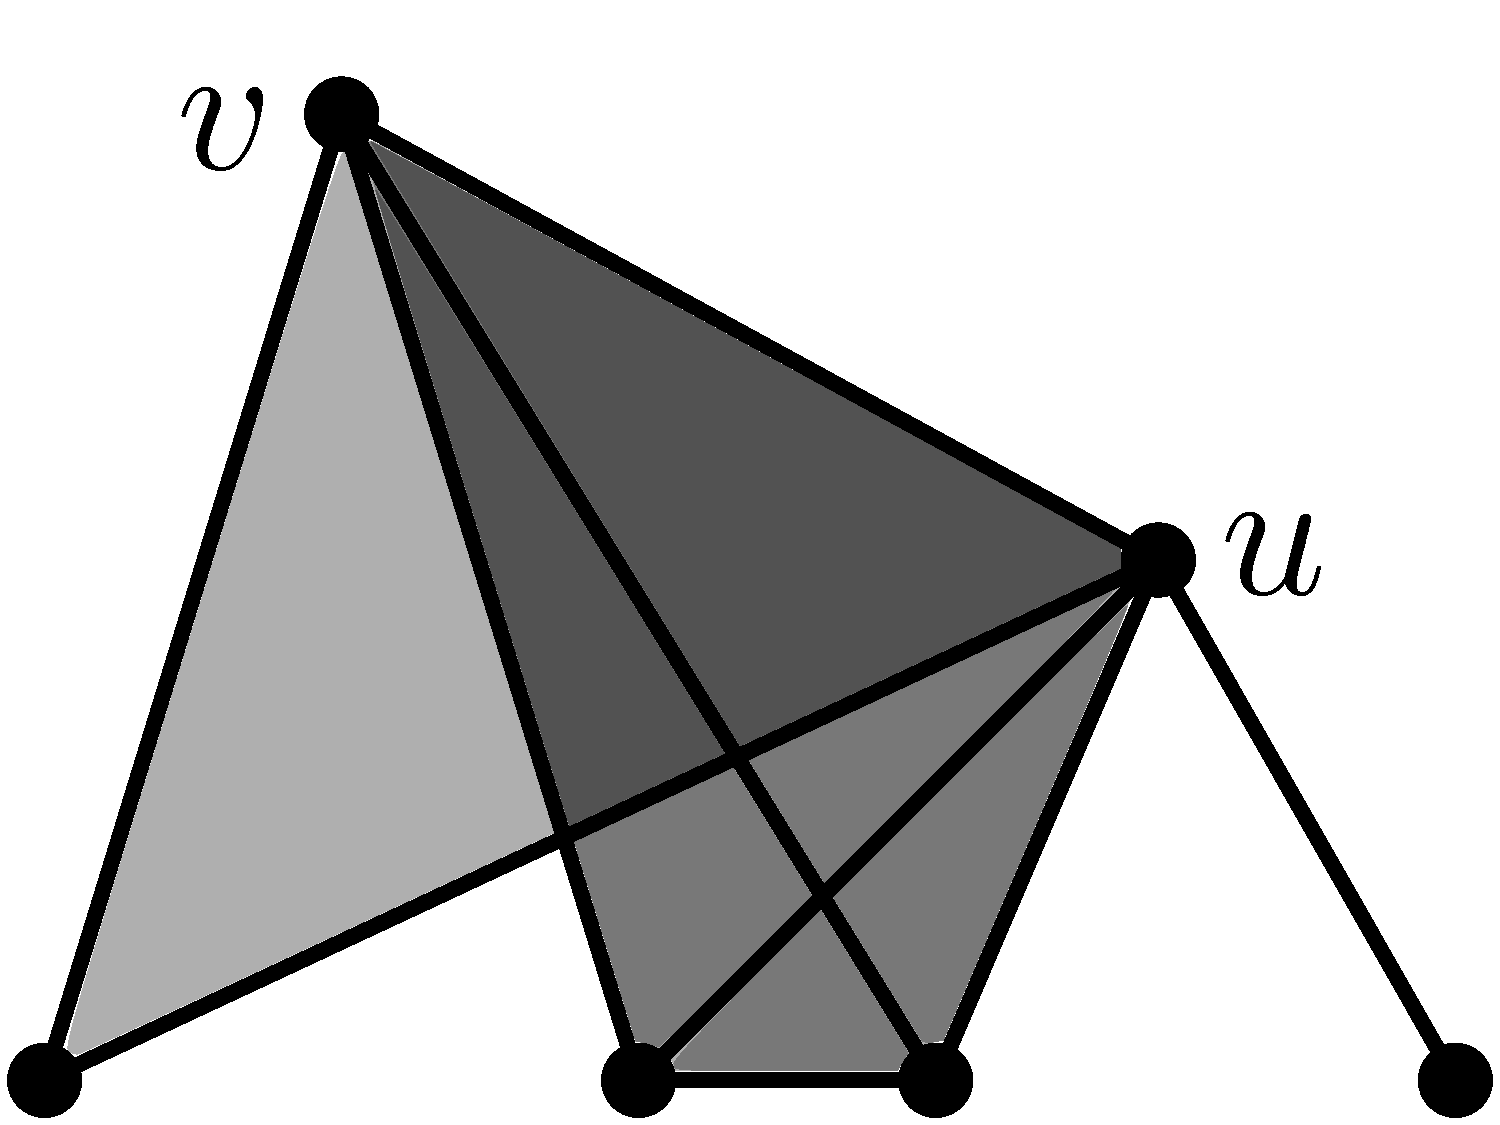
\includegraphics[width=0.2\textwidth]{Dominated2_labeled.pdf}
\hspace{20mm}
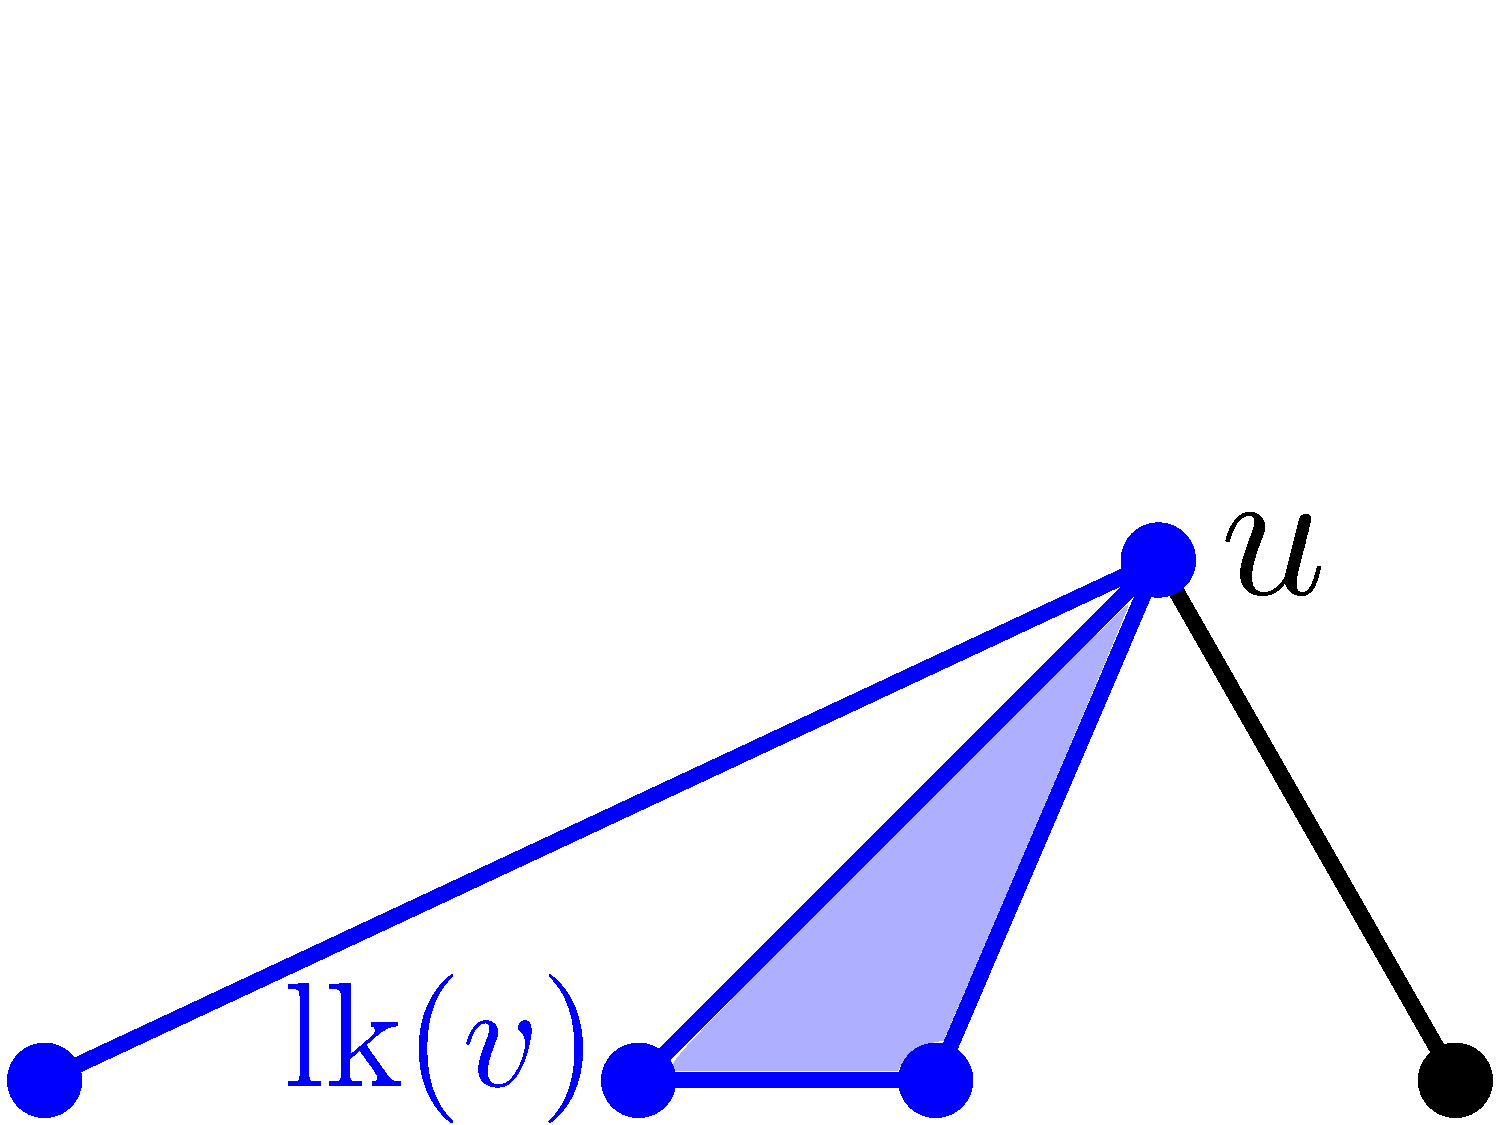
\includegraphics[width=0.2\textwidth]{Dominated4_labeled.pdf}
\caption{(Left) The clique complex $\cl(G)$. (Right) The clique complex $\cl(G\setminus v)$ after the dominated vertex $v$ has been removed. These simplicial complexes have the same shape, topologically speaking.}
\label{fig:dominatedClique}
\end{figure}

Some references for dominated vertices are \cite{BabsonKozlov2006,barmak2012strong,Matouvsek2008}, although those references are perhaps way more complicated than what we need (the notion of dominated vertices for arbitrary simplicial complexes is more complicated than that for clique complexes).


\section{Questions involving topology}

If the clique complex is ever not a wedge sum of spheres, then we have disproved an open conjecture!

If the clique complexes are always wedges of spheres, then by analyzing their cores, we may gain insight on how to prove this conjecture.

In the minimal cores that we generate, are all of the homology generators easy to interpret (using what's known on the circle)?


\section{Simplicial collapses}
\label{sec:collapse}

\note{We should expand this discussion of simplicial collapses.}

\note{Define what it means for a simplex in a simplicial complex to be \emph{maximal}.}

\note{Define simplicial collapses.}

See (\footnote{\url{https://en.wikipedia.org/wiki/Collapse\_(topology)}}) for a description of simplicial collapses!



\section{Punctured simplices}
\label{sec:punctured}

\subsection{Convex sets}

\note{Convex sets in $\R^n$ are a classical topic, that we should define and review in $\R^2$.}

\begin{definition}
\note{Define what it means for a set $S\subseteq\R^2$ to be convex.}
\end{definition}

\begin{definition}
Given a set $S\subseteq \R^2$, its \emph{convex hull} $\conv{\sigma}$ is the intersection of all convex sets in $\R^2$ containing $S$.
\end{definition}

\note{Add a picture of a convex hull in $\R^2$!}

\begin{definition}
Given a finite set $\sigma\subseteq \R^2$, we define its \emph{boundary vertices} to be
\[b(\sigma)=\{x\in \sigma~|~x\in\partial\conv(\sigma)\}\]
to be the set of all points in $\sigma$ that are on the boundary of the convex hull of $\sigma$.
\end{definition}

\subsection{Punctured sets}

\note{Punctured sets are a term that we're ``inventing", definining, and using here for our purposes!}

\begin{definition}
We say that a finite set $\sigma\subseteq \R^2$ is \emph{punctured} if $b(\sigma)\neq \sigma$.
\end{definition}

Note that $\sigma\subseteq \R^2$ is punctured exactly when there exists a point $x\in\sigma$ that is in the \emph{interior} of the convex hull $\conv(\sigma)$.

\note{Add a picture of an example punctured set!}

\subsection{Unpunctured cores}

Let's consider now the main context of this paper, where $X\subseteq \R^2$, and where we're trying to simplify $\cl(G(X))=VR(X;1)$.

If $\sigma\subseteq X$ is maximal, then consider the boundary vertices $b(\sigma)\subseteq \sigma$.
Note that $b(\sigma)$ is contained in a unique maximal simplex of $\cl(G(X))$, namely $\sigma$ \note{this is worth proving}.
Hence if $\sigma$ is punctured, then we can perform a simplicial collapse (Section~\ref{sec:collapse}) to remove all simplices $\tau$ with $b(\sigma)\subseteq \tau\subseteq \sigma$.

\begin{claim}
\label{claim:punctured-maximal}
If a simplicial complex with vertex set $X\subseteq\R^2$ contains a punctured simplex, then it contains a maximal punctured simplex.
\end{claim}

\begin{proof}
\note{True? Prove this!}
\end{proof}

Starting from $\cl(G(X))$ with $X\subseteq\R^2$ finite, we may iteratively perform simplicial collapses with free faces $b(\sigma)$ (with $\sigma$ a maximal punctured simplex) until we obtain a reduced simplicial complex with no maximal punctured simplices.
(Keep in mind that as we perform simplicial collapses, now new simplices become maximal.)
By Claim~\ref{claim:punctured-maximal}, this reduced simplicial complex furthermore contains no punctured simplices!
Let's call such a resulting complex an \emph{unpunctured core} of $\cl(G(X))$.
See Algorithm~\ref{alg:punctured} for more details!

\begin{algorithm}[ht]
\SetAlgoLined
\KwData{Clique complex of unit disk graph $\cl(G(X))$ for $X\subseteq \R^2$
\note{How to store simplicial complexes (\footnote{\url{https://arxiv.org/pdf/1503.07444.pdf}})?}}
\KwResult{An unpunctured core of this simplicial complex}
(1) Determine the maximal simplicies $\sigma$ \newline
(2) Determine the boundary vertices $b(\sigma)$ for each maximal simplex $\sigma$ \newline
(3) Determine if each maximal simplex is punctured \newline 
(4) Preform simplicial collapse with the convex hull of the punctured simplex as a free face\newline 
(5) Loop to (1)
\caption{Computing an unpunctured core}
\label{alg:punctured}
\end{algorithm}



\subsection{Properties of unpunctured cores}

\begin{question}
\label{ques:unpunctured-core}
Let $\cl(G(X))$ be the clique complex of the unit disk graph of $X\subseteq \R^2$. Let an ``unpunctured core" be the resulting simplicial complex after removing all maximal punctured simplices, i.e., after applying Algorithm~\ref{alg:punctured}.
Is it true that any two unpunctured cores of $\cl(G(X))$ are isomorphic?
\note{Wait, maybe there is a unique unpunctured core, period! Meaning it's unique not only up to isomorphism, but also up to equality!}
\end{question}

If the answer to the above is ``yes", then this would be analogous to the fact that any two minimal cores of a graph are isomorphic!

If the answer to the above question is ``yes", then this is saying that the order via which we remove punctured simplices in Algorithm~\ref{alg:punctured} doesn't really matter!

\subsection{Dividing the plane into ``regions" based on the maximimal (unpunctured) simplices in an unpunctured core!}

\subsection{``Long edges"}

Next remove all free edges, i.e., edges that are contained in a unique maximal simplex?
Unless this edge is on the boundary (of the projection of the complex to $\R^2$), then this maximal simplex will be a tetrahedron or larger, and hence the free edge will be crossing another edge.
This likely means that we can always choose to remove a non-Delaunay free edge (the Delaunay edges should be kept, and no two Delaunay edges cross).
\note{This might be a good place to do computational experiments!}

After removing all punctured simplices as in the above subsection, we still have a lot of long edges (note edges are punctured with probability zero, i.e.\ edges are never punctured if the points are in general position).
Is there a nice way to remove these long edges?
As a starting case, think of two long crossing diagonal edges (of a quadrilateral) which hence form a tetrahedron --- can we use this tetrahedron to collapse away one of these two long edges, getting down instead to two triangles?



\section{Other notions of ``collapse" in topology}\label{sec:collapse}

(Besides removing dominated vertices)

Last meeting (2/11/19) we talked about the idea that removing dominated vertices may not be enough to fully understand our conjecture. Here is a list of other homotopy-preserving operations that may or may not be of use to us. Many of these relate to the Vietoris-Rips complex, which is a generalization of the unit disk graph. In particular, when our points are sampled from $\R^2$ equipped with the Euclidean metric and $\delta=1$, the Vietoris-Rips complex is the clique complex of the unit disk graph.

\begin{itemize}
\item \textbf{$\varepsilon$-Crushing} \\
Given a Vietoris-Rips complex, how else can we remove vertices in a homotopy preserving way? One answer may be $\varepsilon$-crushing, highlighted in the article by Latschev~\cite{Latschev2001}.
In particular, the flat case in section 2 may be of use. 
If anyone could determine whether or not this can help us simplify our complexes or if it is simply a generalization of removing dominated vertices, that would be helpful!
\item \textbf{The Rips Shadow} \\
Another way to simplify the Vietoris-Rips complex is to calculate its shadow, or its projection down onto the plane.
The article by Chambers gives isomorphisms between certain homotopy groups of the Rips complex and its shadow~\cite{Chambers2008}. It also includes algorithms for computing the shadow, for those who are more programming-minded.

\item \textbf{s-Dismantlability} \\
In a general flag or clique complex, where every simplex corresponds to a complete subgraph of its 1-skeleton, we can define a notion of s-dismantlability.
A vertex $v_i$ is considered \textit{s-dismantlable} in $G$ if the subgraph $N_{G}(v_i)$ of the neighbourhood of $v_i$ is dismantlable.
Boulet et al.\ show that s-dismantlability can be used to define more homotopy preserving collapses such as edge deletion, even if the vertex isn't dominated~\cite{Boulet2010}.

\item \textbf{Other Collapses} \\
In a simplicial complex, there are other operations that collapse edges and vertices while preserving homotopy types. Attali et al.\ begin by defining an \textit{elementary collapse} as a method of removing two vertices, then generalize it to \textit{classical collapses, extended collapses} and \textit{generalized collapses}~\cite{Attali2013}.
They then apply these collapses in certain orders to define various reduction sequences for common cases.
\item Does replacing a simplicial complex with its (homotopy equivalent) nerve, as described in~\cite{barmak2012strong}, ever help, for instance after having already removed all punctured simplices?
\end{itemize}




\bibliographystyle{plain}
\bibliography{minimalCores}

\end{document}
